%!TEX root = ../thesis.tex

\begin{savequote}[70mm]
	The Internet is becoming the town square for the global village of tomorrow.
	\qauthor{Bill Gates}
\end{savequote}


\chapter{Technologies}\label{chapter:technologies}
	
	This chapter explains more in detail the underlying technologies of this project.
	Starting from the general definition of a network and the most common architectures, radio technologies and micro-controllers.
		
	\section{Fundamentals of network communication}
		
		\begin{center}
			\begin{minipage}[H]{0.9\columnwidth}
				\begin{center}
					``\textit{A computer network is a structure that makes available to a data processing user at one place some data processing function or service performed at another place.}'' \cite{nla.cat-vn252493}
				\end{center}
			\end{minipage}
		\end{center}
	
		Starting from the definition of a computer network by Paul E. Green, it is easy to understand its importance in today's society.
		Smartphones, personal computers and other interconnected devices have become omnipresent in modern society, where people have the urge to be connected to each other via these devices.
		% https://www.irishtimes.com/business/online-services-playing-more-important-role-in-everyday-activities-1.511857
		Not only they are used for fun, leisure and other social activities, but they allow connection to services such as online banking, government services and healthcare, which require a stable and secure connection among the systems they use in order to provide a safe experience for their users.
		All this to say, networks are everywhere underneath today's technology.
		There are no services or devices that can stand on their own without sharing data to other devices, to synchronize and provide a better user experience, to get updates from the manufacturer or simply to send a keep-alive message.
		
		While this raw data is important for computers, people, the final users, process it to gain information, and this exchange of information from all around the world has brought radical changes many levels, from a cultural and economical point of view.
		The possibility of having a network to share information is the next step of globalization, which started with the trade of goods among countries and now brings everyone together, allowing for a cultural exchange that lets people unite across the globe.
		
		This big network that is used to exchange information all around the world has a special name: Internet.
		% https://en.wikipedia.org/wiki/Right_to_Internet_access	
		% https://www.diplomacy.edu/blog/right-access-internet-countries-and-laws-proclaim-it/
		Many countries, such as Finland, Spain and Greece, have recognized the importance of this network and have given people the ``\textit{right to Internet access}'', also known as the \textit{right to broadband} or \textit{freedom to connect}.
		In these countries, service providers must be able to supply a mandatory minimum connection capability to all desiring home users in the regions of the country they serve.
		
		% http://www.redbooks.ibm.com/abstracts/gg243376.html
		It is important to note that \textit{Internet}, with a capital \textit{I}, is a particular set of worldwide interconnected networks \cite{gg243376}, but a common network of networks is called \textit{internetwork}, shortened by internet, with a lowercase \textit{i}.
		
		Such distinction began in the 1980s and has been described in RFCs\footnote{ \href{datatracker.ietf.org/doc/html/rfc871}{RFC 871 (1982): A PERSPECTIVE ON THE ARPANET REFERENCE MODEL}}$^{,}$\footnote{ \href{datatracker.ietf.org/doc/html/rfc872}{RFC 872 (1982): TCP-ON-A-LAN}} by computer scientists that understood how ARPANET was expanding and its dimensions were not enough anymore to accommodate the amount of data traveling from one computer to another.
		% https://en.wikipedia.org/wiki/Commodore_64
		At that time, computers such as the \textit{IBM 5150} and the infamous \textit{Commodore 64} were starting to become more and more available, even if highly priced, not only to companies and universities, but also to consumers who brought them in their households, especially with the advent of \textit{MS-DOS}, the dominant operating system throughout the 1980s, now open-source\footnote{ \url{www.github.com/microsoft/MS-DOS}}.
		
		As described by IBM in one of their technical books from the time, ''\textit{it is possible to divide the Internet such as the following groups of networks}'' \cite{gg243376}:
		\begin{itemize}
			\item \textit{backbones}: large and strategical data routes among core networks and routers that compose and connect the Internet;
			\item \textit{regional networks}: that connect large facilities such as universities and colleges;
			\item \textit{commercial networks}: that provide to their subscribers access to the Internet;
			\item \textit{local networks}: which run, for example, across a campus university or private property.
		\end{itemize}

		Given this increase of computers connecting to the Internet, there came the need for a revised structure that could better organize these components in a more robust, but also flexible, large network.
		With more accessible operating systems, such as \textit{Windows 95} and \textit{Windows 98}, and the advent of Tim Berners-Lee's \textit{World Wide Web} (or \textit{WWW}), computers became a common commodity.
		The invention of the web and its ease to navigate, using hyperlinks and search engines, culminated in the \textit{dot com} bubble, a stock market bubble in the late 90s that caused rapid rise of technology companies in stock market.
	
		\begin{figure}[H]
			\centering
			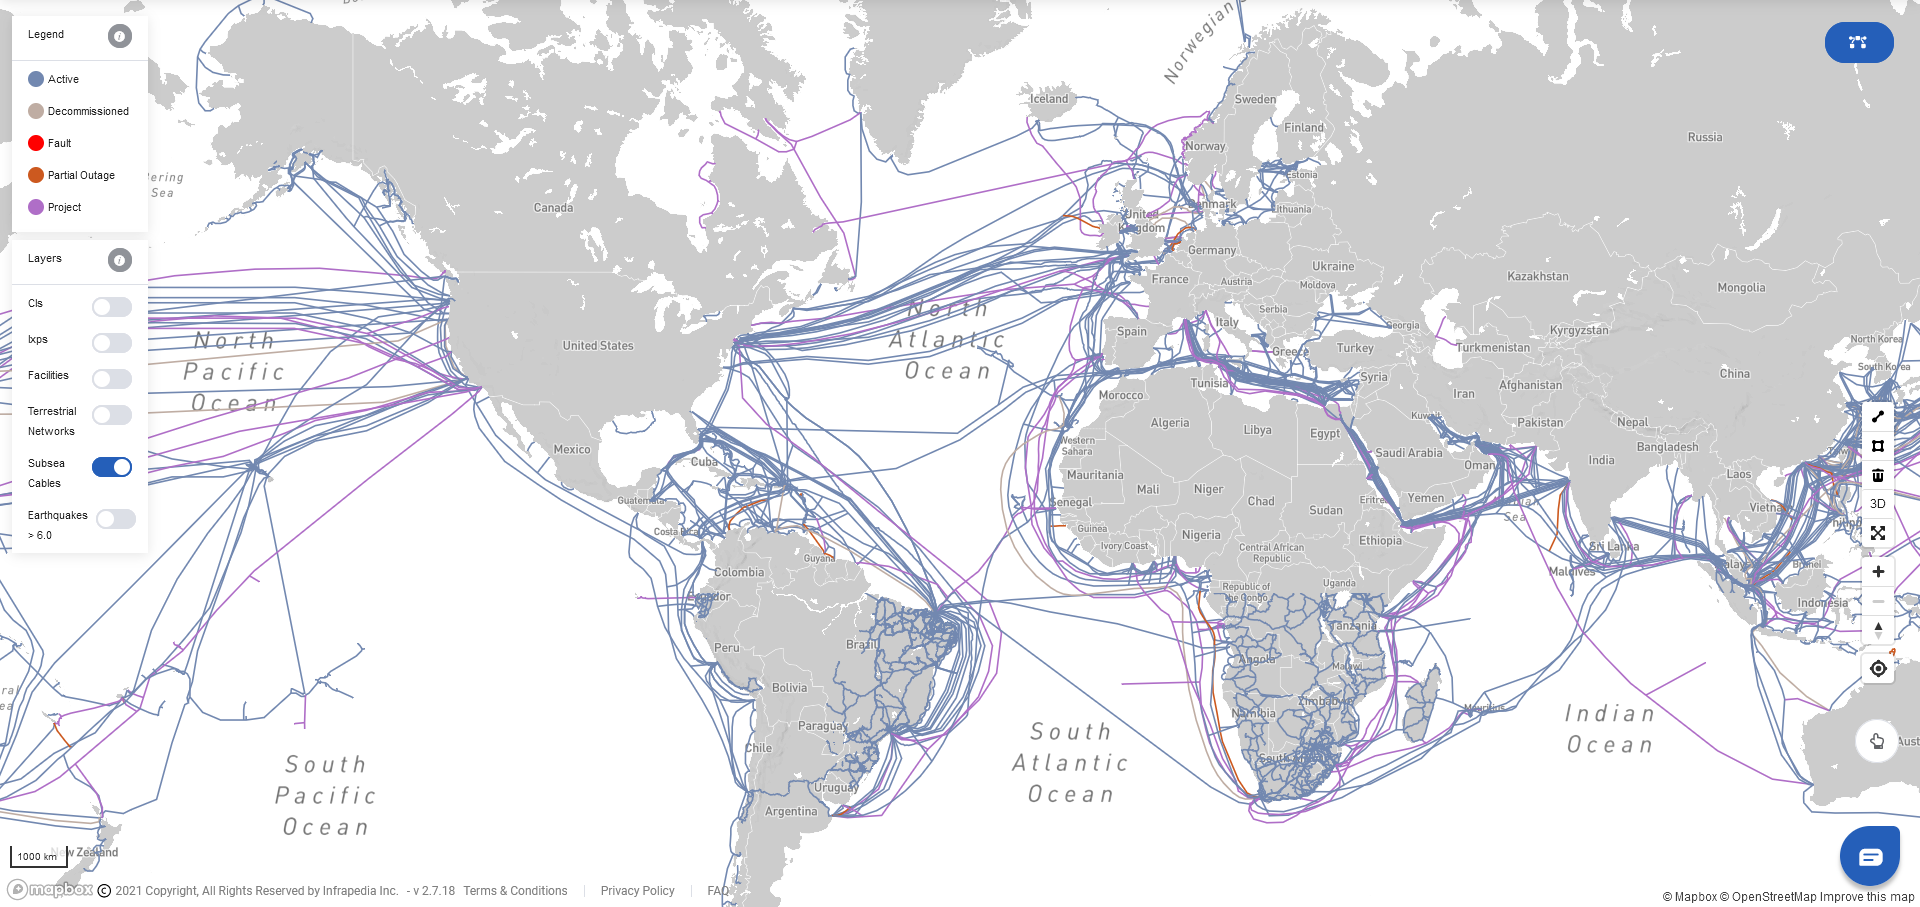
\includegraphics[width=\textwidth]{resources/img/chap3/backbone}
			\caption[Subsea Internet backbone cables between US and Europe]{Subsea Internet backbone cables between US and Europe\footnotemark}
		\end{figure}
		\footnotetext{~\url{https://www.infrapedia.com/app}}
	
		Networks can be categorized based on the area they cover and serve:
		\begin{itemize}
			\item \textit{Wide Area Network}, or \textit{WAN}: also called long haul networks, provide communication over long distances;
			% https://www.cloudflare.com/learning/network-layer/what-is-a-metropolitan-area-network/
			\item \textit{Metropolitan Area Network}, or \textit{MAN}: provide communication inside a metropolitan area, which could be a single large city, multiple cities, or any given large area with multiple buildings;
			\item \textit{Local Area Network}, or \textit{LAN}: provide the highest speed connections among computers in a small and circumscribed area;
			% https://www.cloudflare.com/learning/network-layer/what-is-a-personal-area-network/
			\item \textit{Personal Ara Network}, or \textit{PAN}: connects devices within a user's immediate area.
		\end{itemize}
	
		Another level of distinction among networks, which is made based on the power consumed by the transmission medium, is explained in Section~\ref{sec:radio_tech}.
		
		Since now everyone can connect to the Internet and access its services, there is no need for the average user to understand what happens between his machine and the rest of the network, which means he only sees the information displayed, without knowing where it arrives from or what path it took to arrive on his monitor.
		
		For computer scientists though, it is important to understand the difference between \textit{network architecture} and \textit{network topology}.	
		A \textit{network architecture}, as described by by Paul E. Green, ``\textit{is a complete definition of all the layers necessary to build the network}'' \cite{nla.cat-vn252493}.
		This is focused on the network software, which needs to be highly structured in order to allow for heterogeneous systems to communicate with each other.
		% https://standards.iso.org/ittf/PubliclyAvailableStandards/s020269_ISO_IEC_7498-1_1994(E).zip
		One example of network architecture is the \textit{ISO/OSI reference model}\footnote{ \url{www.iso.org/standard/20269.html}}, which is implemented by the \textit{TCP/IP protocol stack}.
		
		% https://stackoverflow.com/questions/38596488/in-which-layer-is-http-in-the-osi-model
		\begin{figure}[h]
			\centering
			\includegraphics[width=\textwidth]{resources/img/chap3/isoosi}
			\caption{The ISO/OSI reference model against the TCP/IP protocol stack}
		\end{figure}
		
		Thus comes the definition of a protocol as ``\textit{a set of agreements for interaction of two or more parties and is expressed by three components, syntax (e.g., a set of headers, a set of commands/responses), semantics (the actions and reactions that take place, including the exchange of messages), and timing, the sequencing and concurrency aspects of the protocol}'' \cite{nla.cat-vn252493}.
		Different types of network use distinct architectures, based on the transmission medium and how well this performs (errors, speed, etc.).
		
		% https://www.omnisci.com/technical-glossary/network-topology
		On the other hand, the \textit{network topology} refers to the manner in which the links and nodes of a network are arranged to relate to each other.
	
		\textbf{\textcolor{red}{\hl{// To be completed w/ definition of UNICAST / MULTICAST / BROADCAST}}}
		
		As shown in Figure~\ref{img:network_topologies}, some of the most common network topologies are:
		\begin{itemize}
			\item \textit{point-to-point}: in which devices are connected directly;
			\item \textit{bus}: devices are connected to each other via a backbone cable;
			\item \textit{ring}: two dedicated point-to-point links connect a device to the two devices located on either side of it, creating a ring of devices through which data is forwarded via repeaters until it reaches the target device;
			\item \textit{star}: connects each device in the network to a central hub. Devices can only communicate with each other indirectly through the central hub;
			\item \textit{tree}: parent-child hierarchy in which star networks are interconnected via bus networks;
			\item \textit{mesh}: a dedicated point-to-point link connects each device on the network to another device on the network, only carrying data between two device;
			\item \textit{hybrid}: any combination of two or more topologies.
		\end{itemize}
	
		An important factor that decides the industrial acceptance of any network topology is its ``\textit{scalability}'', concept reiterated in Section~\ref{sec:scalability} for mesh networks.
	
		\begin{figure}[h]
			\centering
			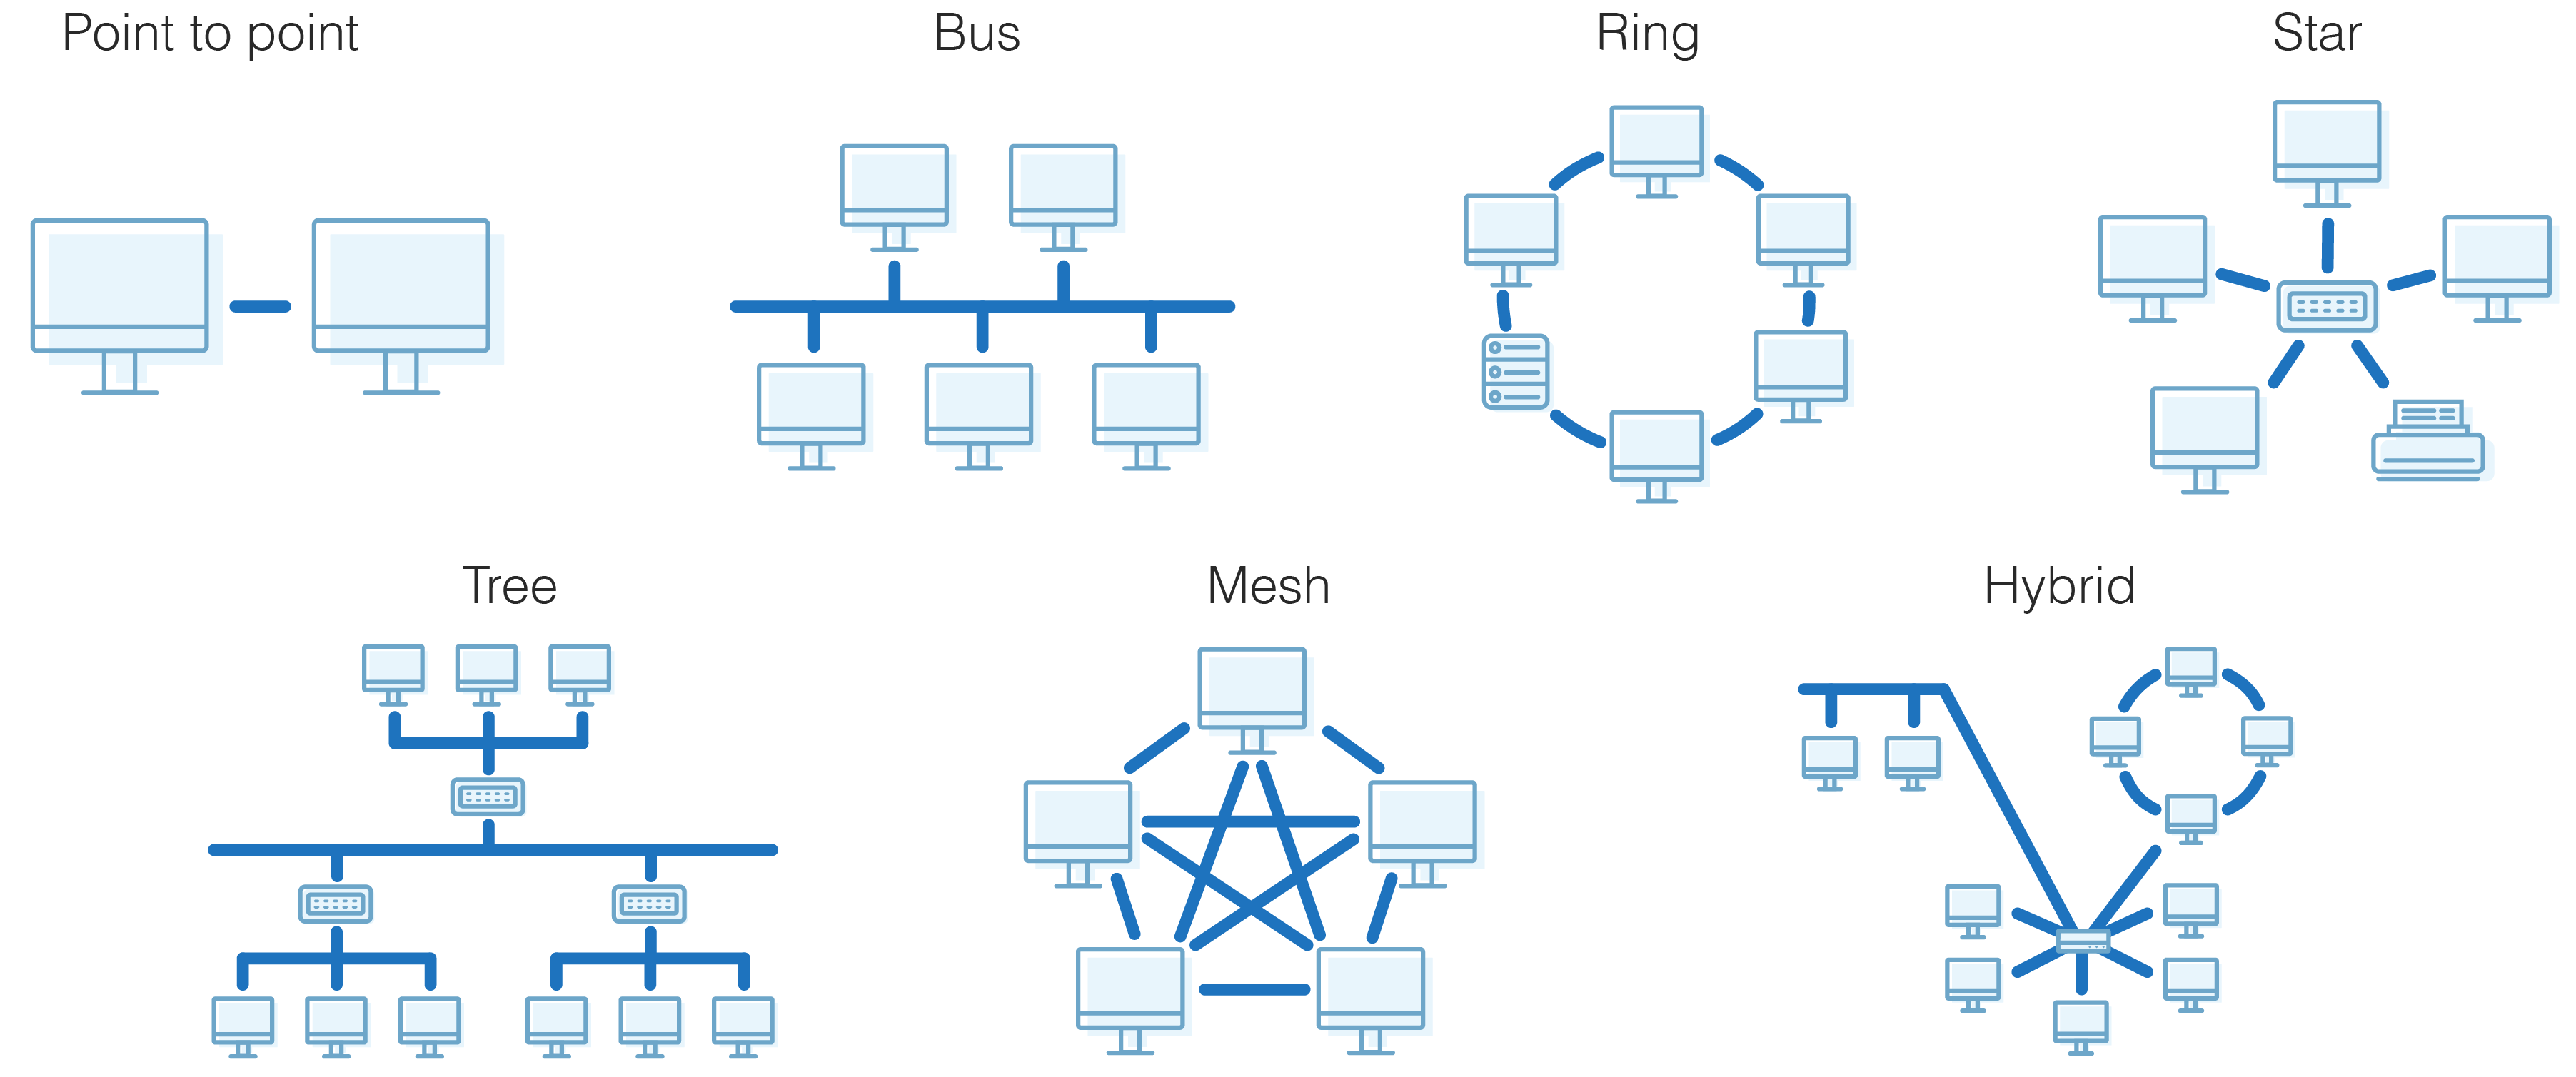
\includegraphics[width=\textwidth]{resources/img/chap3/network_topologies}
			\caption{Common network topologies}
			\label{img:network_topologies}
		\end{figure}
	
		The project presented in this thesis regards a network with a mesh topology, which can be considered a \textit{multi-hop network}, since data passes from node to node until it reaches its destination.
		This is better described in Chapter~\ref{chapter:proposed_solution}, alongside the technical details of mesh proposed in this thesis, which has a span of LAN / MAN, since it connects devices that are in a circumscribed area but can be also placed further from each other, in order to cover longer distances.
			
		The organization responsible for Internet standards is the Internet Engineering Steering Group (IESG)\footnote{ \url{www.ietf.org/about/groups/iesg}}.
		It is necessary to have an organization looking over the Internet itself since it gives the regulations that allow all devices to interconnect with each other.
	
	\section{Radio technologies}\label{sec:radio_tech}
		
		% https://en.wikipedia.org/wiki/Invention_of_radio
		Although Guglielmo Marconi is usually credited as the inventor of radio due to the creation of the first commercially successful wireless communication system \cite{4137304}, many scientists before him have studied the subject of radio waves.
		The discovery of electromagnetic waves, including radio waves, by Heinrich Rudolf Hertz in the 1880s, came after theoretical development on the connection between electricity and magnetism that started in the early 1800s.
		Scientists tried to achieve the idea of a wireless telegraph via electric conduction and electromagnetic induction for a while before the establishment of radio-based communication.
		
		% https://science.howstuffworks.com/innovation/inventions/who-invented-the-radio.htm
		Other important experiments were made by Nikola Tesla, who invented the \textit{Tesla coil}, a device essential to sending and receiving radio waves, during efforts to develop a ``wireless'' lighting system.
		This Tesla coil has been used by Marconi in his experiments and is present in the patent he presented for radio transmission of data.
		
		More than a century later, radio technology has massively evolved and is used on a daily basis.
		Devices has shrunk in dimension and the amount of transmission meanings have increased far from what both Tesla and Marconi could have thought of.
		Thus, in order to give a complete picture of radio transmitting technologies, it is important to make a distinction among the ones that are made for internal or nearby use compared to the ones which are used for longer distances.
		
		% https://sites.google.com/site/pnutpck11/lesson-9---wireless-transmission-media
		Many users opt for wireless transmission media because it is more convenient than installing cables, even if they might sacrifice some performance. 
		Also, using wireless technology allows transmission in locations where it is impossible to install cables.
		Types of wireless transmission media used in communications include:
		\begin{itemize}
			\item \textit{infrared}: wireless transmission medium that sends signals using infrared light waves;
			\item \textit{broadcast radio}: wireless transmission medium that distributes radio signals through the air over long distances such as between cities, regions, and countries and short distances such as within an office or home.
			Bluetooth, UWB, Wi-Fi, and WiMAX communications technologies use broadcast radio signals;
			\item \textit{cellular radio}: form of broadcast radio that is used widely for mobile communications, specifically wireless modems and cell phones, which use high-frequency radio waves to transmit voice and digital data messages;
			\item \textit{communications satellite}: space station that receives microwave signals from an earth-based station, amplifies (strengthens) the signals, and broadcasts the signals back over a wide area to any number of earth-based stations.
			Applications such as air navigation, television and radio broadcasts, weather forecasting, video conferencing, paging, global positioning systems, and Internet connections use communications satellites.
		\end{itemize}
		
		With new transmission technologies, new network architectures and topologies that are better suited for the transmission method have emerged.
		Topologies that bring computation closer to the edge are also rising in popularity, since they allow for faster computation and they bring data closer to the user.
		These are Cloud, Edge and Fog Computing, as mentioned in Chapter~\ref{chapter:background}.
		
		LAN, MAN and WAN are not enough anymore to describe the new topologies.
		An important distinction is now made by other factors such as power consumption, cost of the devices and range of transmitter and receiver.	
		The most important new category of wireless communication, that interests IoT and represents a large portion of the market at the time of writing, as described in Chapter~\ref{chapter:background}, is \textit{LPWAN}, which stands for \textit{Low Power Wide Area Networks} and is composed by nodes that are capable of \textit{long range communication}, \textit{low power consumption} and \textit{low cost}.
		Lightweight protocols also allow reducing complexity in hardware design and lower device costs.
		Its long range combined with a star topology reduces expensive infrastructure requirements, and the use of license-free or licensed bands reduces network costs.
		Growing popularity of IoT use cases in domains that rely on connectivity spanning large areas and the ability to handle a massive number of connections is driving the demand for LPWAN access technologies \cite{fi12030046}, and the project presented in this thesis falls under this category of communication.
		LPWAN allows connectivity in many applications, from crowded areas in smart cities to smart farming and smart environment, from security and emergencies to e-health.
		
		Various wireless transmission methods can be used to create a LPWAN, some of the most used in IoT are Sigfox, LoRa and NarrowBand IoT (NB-IoT).
		In Subsection \ref{subsec:lora_lorawan}, follows a more complete explanation on LoRa and LoRaWAN.
		One crucial factor for these transmission methods is to ``\textit{support a massive number of simultaneously connected devices with low data rates}'' \cite{fi12030046}.
		
		Other important communication technologies in IoT are RFID, NFC, for contact purposes, Bluetooth, Zigbee for a personal network and IEEE 802.11, or Wi-Fi, for a local area.
		The latter was used in the ArduEco project, described in Sec. \ref{subsec:ardueco}.
		Fig. \ref{img:wireless_coverage} contains a representation of the geographic coverage in meters of the various aforementioned wireless transmission methods.
	
		% \newpage
		\begin{figure}
			\centering
			\includegraphics[width=\textheight,height=\textwidth,keepaspectratio,angle=90]{resources/img/chap3/iot_range}
			\caption[Wireless access geographic coverage]{Wireless access geographic coverage \cite{fi12030046}}
			\label{img:wireless_coverage}
		\end{figure}
		% \newpage
	
		\subsection{LoRa and LoRaWAN}\label{subsec:lora_lorawan}
	
			\textit{LoRa} (short for \textit{long range}) is a spread spectrum modulation technique derived from the \textit{chirp spread spectrum} (\textit{CSS}) technology.
			LoRa devices provide a long range, low power wireless platform that is being widely adopted for the IoT networks worldwide.
			In conjunction with the LoRaWAN protocol, LoRa devices enable smart IoT applications in various contexts, like: energy management, natural resource reduction, pollution control, infrastructure efficiency, disaster prevention, and more. 
	
			LoRaWAN, on the other hand, is a comprehensive network architecture that details a LPWAN technology.
			It was designed to interconnect battery operated ``things'' and provides a bi-directional communication service with end-to-end security features.
	
			The architecture is based on a star-of-stars topology in which specific devices called gateways relay messages between end-devices and a central network server.
			The wireless communication takes place through a single-hop link between the end-device and one or many gateways.
			The specification defines the device-to-infrastructure physical layer parameters (LoRa) and the specific LoRaWAN protocol to allow for full interoperability among manufacturers.
			It defines the technical implementation but it does not define any commercial model or type of deployment, e.g., public, shared, private, enterprise. 
			
			The LoRaWAN specification is developed and maintained by the LoRa Alliance, an open association of collaborating members. 
			With LoRa and LoRaWAN the intention was to provide the possibility to deploy Internet of Things applications fast in areas where large distances are involved, yet low bandwidth is needed.
			
			Low bandwidth makes it ideal for practical IoT deployments with less data or where data transmissions are not constant, for example with waste management where the information that is required is whether a waste bin is full or not.
			Moreover, the \textit{end-to-end} delay (or the \textit{RTT}, \textit{Round-Trip-Time}) can be relatively high, with values below one second being acceptable.
			
			Conversely, packet loss is a more crucial factor.
			In LoRaWAN, once a message has been delivered, there is no acknowledgement of receipt.
			However, nodes can request acknowledgements.
			In this case, if many gateways receive the same packet, the cloud has to choose one gateway to respond
			at a fixed time, usually a couple of seconds later.
			The problem is that when a gateway is transmitting back to the node, it stops listening to everything else.
			So, if an application needs a lot of acknowledgements, the gateway will very likely spend more time transmitting acknowledgements than listening, which will eventually lead to a network saturation.
			
			Therefore, classical applications do not require acknowledgments and that's why having a reliable network with very small packet loss rate is crucial to not lose relevant information.
			
			Chirp spread spectrum has been used in military and space communication for decades due to the long
			communication distances that can be achieved and robustness to interference, but LoRa is the first low cost implementation for commercial usage.
			
			\begin{figure}[h]
				\centering
				\includegraphics[width=\textwidth]{resources/img/chap3/LoRa_Why_Range}
				\caption{Range of LoRa transmission compared to Wi-Fi, BLE and Cellular}
				\label{img:lora_range}
			\end{figure}
			
			The advantage of LoRa is in the technology's long range capability, as can be seen in Figure~\ref{img:lora_range} and in Figure~\ref{img:wireless_coverage}.
			Range highly depends on the environment or obstructions in a given location, but LoRa and LoRaWAN have a link budget greater than any other standardized communication technology.
					
	\section{Hardware (Microcontrollers)}\label{sec:microcontrollers}
	
		% Parlare di board come questa?
		% https://www.kickstarter.com/projects/sodaq/loraone-the-lora-iot-development-board?ref=discovery&term=lora%20mesh
	
		Microcontrollers (or MCUs, short for Microcontroller Unit) are compact integrated circuits designed to fit in specific environments or to perform specialized functions, which usually do not require any particular computation, memory capacity or power.
		This has been made possible thanks to the continuous shrinking of transistors, which makes almost all the components more compact, and the improved power sources.
		In junction with the previously described wireless technologies, microcontrollers are at the hearth of IoT devices, described in Chapter~\ref{chapter:background}, and they require long-lasting, low-cost, and sustainable batteries.
		
		The number of IoT connected devices is expected to grow up to 75 billion worldwide by 2025 \cite{statista}, and connection density is expected to be one million devices per square Km \cite{noma}.
		Hence, these devices will generate massive data and consume significant energy.
		
		Given the amount of specific functions an MCU can perform, there are many boards on the market.
		Some are very alike, while others are very different, since they are expected to be used in other types of environments.
		All boards consist on a similar architecture, which contains the processing unit (CPU), along with memory and programmable input/output (or I/O) peripherals.
		
		\begin{figure}[H]
			\centering
			\includegraphics[width=\textwidth]{resources/img/chap3/generic_board}
			\caption{Attiny 85 on the left, in the middle two boards based on the ESP32, on the right the Asus Tinker Board 2}
			\label{img:generic_board}
		\end{figure}
	
		% https://en.wikipedia.org/wiki/Microcontroller
		In Figure~\ref{img:generic_board}, there are four different boards, the one farthest on the left is the \textit{ATtiny 85}\footnote{ \url{www.microchip.com/en-us/product/ATTINY85}}, a low-power, 8-bit microcontroller that is made for general purpose and can be programmed for easy tasks, from simple LEDs flashing, to more ``\textit{elaborate}'' small sensor projects.
		% https://en.wikipedia.org/wiki/ESP32
		The two boards in the middle are based on the ESP32 chip, a series of low-cost, low-power system on a chip microcontrollers with integrated Wi-Fi and dual-mode Bluetooth.
		They both are more powerful compared to the ATtiny 85, and the right one offers an integrated LoRa antenna on board.
		Far on the right, there is the Asus Tinker Board 2\footnote{ \url{https://tinker-board.asus.com/product/tinker-board-2.html}}, a board powered by an Arm 6-core system on a chip (SoC), with a 64-bit Armv8 architecture.
		This board provides much more computing power compared to the previous ones and is able to run operating systems such as Linux and Windows.
		
		% https://www.amazon.it/Meipai-ATTINY85-20PU-ATTINY85-chip-ATMEL/dp/B08HPPMJ52/
		% https://www.amazon.it/AZDelivery-NodeMCU-Development-Arduino-gratuito/dp/B071P98VTG/
		% https://www.amazon.it/Scheda-Modulo-Wireless-T-Beam-Batteria/dp/B07X2KPN4L/
		% https://www.welectron.com/navi.php?qs=Tinker
		One of the strong points of these boards is the price: the ATtiny is priced around $1$€ when bought in bulk, the boards on the middle cost around $7$€ and $15$€ respectively, while the board by Asus is the most expensive of the four and starts from $70$€.
		
		It is important to note though that using a generic board in a production environment might not be ideal, since it might lack of customer support and documentation from the company.
		The boards described subsequently are from three of the major MCU producers, Arduino, Raspberry Pi and Pycom, which have built hardware that is well documented and suited for many different environments, from hobbyists to industrial use.
		
		The simplified architectures and the constraints of embedded devices are reflected in the narrow choice for programming languages.
		It is hard to find an MCU programmed in Java since this would require the JVM running in the background.
		Popular languages for MCUs are, for example, C/C++, Assembly, Rust, Ada, Erlang, \textit{etc.}
		All these have in common the fact that they are compiled and the bytecode has a small footprint.
		A particular microcontroller company, Arduino, has developed a version of C++ specific for their boards, but given the simplicity of this new dialect, many boards on the market can be programmed with it.
		Arduino is explained further in Subsection \ref{subsec:arduino}.
	
		Another programming language that is quickly taking hold at the time of writing, is Mycropython.
		As explained in their website it is an ``\textit{efficient implementation of the Python 3 programming language that includes a small subset of the Python standard library and is optimised to run on microcontrollers and in constrained environments}''\footnote{ \url{www.micropython.org}}.
		% https://itqna.net/questions/437/what-definition-verbose-code-and-why-it-interesting-reduce-i
		Python's fast learning curve and talkative code advantages are reflected in this smaller version, available for most microcontrollers.
		
%		Below is a table with the specifications of microcontrollers from Arduino, Raspberry Pi and Pycom, which are better described in the following subsections.
%		\begin{table}[tbp]
%			\begin{center}
%				\begin{tabularx}{\textwidth}{@{}|Y|Y|Y|Y|Y|Y|@{}} 
%					\hline
%					& Arduino UNO R3 & Arduino Nano BLE & Raspberry Pi & Rasperry Pi Pico & Pycom FyPy \\\hline
%						CPU &&&&& \\\hline
%						RAM &&&&& \\\hline
%						ROM &&&&& \\\hline
%						IO PINS &&&&& \\\hline
%						PORTS &&&&& \\\hline
%				\end{tabularx}
%				\caption{Specifications of Arduino, Raspberry Pi and Pycom microcontrollers}
%				\label{table:1}
%			\end{center}
%		\end{table}
	
		\subsection{Arduino}\label{subsec:arduino}
		
			% https://www.arduino.cc/en/Main/AboutUs
			% https://www.oreilly.com/library/view/arduino-a-technical/9781491934319/ch01.html	
			Arduino is a company founded by Massimo Banzi \textit{et al.} in Ivrea, Italy, in 2005, and has released the first commercially available microcontroller.
			They wanted a device that was simple, easy to connect to various ``\textit{things}'' (such as relays, motors, and sensors), and easy to program, besides being inexpensive.
		
			They selected the AVR family of 8-bit microcontroller devices from Atmel and designed a self-contained circuit board with easy-to-use connections, wrote bootloader firmware for the microcontroller, and packaged it all into a simple \textit{Integrated Development Environment} (\textit{IDE}) that uses programs called ``\textit{sketches}'' and Arduino was the result.
			
			The most famous version of their board is the \textit{UNO} (\textit{one} in English).
			Arduino UNO, the one on the left in Figure~\ref{img:arduino_board}, is the most used and most documented board of the whole Arduino family, even if this board does not have any integrated sensors or particular ports for peripherals.
			At the time of writing, the current revision of the board is the Arduino UNO Rev 3\footnote{ \url{https://store.arduino.cc/products/arduino-uno-rev3}}, which consists of 14 digital pins, 6 analog inputs, a power jack and USB connection.
			
			% https://www.circuito.io/blog/arduino-code/
			The Arduino family of products can be programmed in a particular programming language based on C/C++, using a special open-source IDE.
			Arduino was so disruptive in the market that many boards, included the ones in Figure~\ref{img:generic_board}, support the special C++ dialect.
			
			% https://store.arduino.cc/products/arduino-uno-rev3
			% https://store.arduino.cc/products/arduino-yun-rev-2
			% https://store.arduino.cc/products/arduino-nano-33-ble
			\begin{figure}[H]
				\centering
				\includegraphics[width=\textwidth]{resources/img/chap3/arduino_types}
				\caption{Arduino UNO Rev 3 on the left, Arduino Yún in the middle, Arduino Nano 33 BLE on the right}
				\label{img:arduino_board}
			\end{figure}
	
			\textit{Shields} are modular circuit boards that can be added to extend capabilities to different application needs.
			These can be attached directly on top of the board and provide sensors, interfaces, peripherals on a single board, rather than attaching to the Arduino singularly.
			% https://learn.sparkfun.com/tutorials/arduino-shields
			Some of the functionalities that can be added by a shield are Ethernet, Wi-Fi, GPS, displays and cameras, motor drivers.
			Most of the additional shields on the market have been developed for the Arduino UNO, since it is the most common board.
			
			The choice of making the Arduino schematics open-source and accessible to anyone has largely favored the development of newer boards, similar in capacity to the Arduino but more specialized, since producers and board makers are able to keep only the components needed or add different ones.
			An example can be the two middle boards in Figure~\ref{img:generic_board}, which rode the wave of Arduino's popularity.
			Not only the datasheets are available for all boards, but also the Arduino IDE software is open-source.
			
			% https://www.circuito.io/blog/arduino-code/
			The versatility of Arduino and its easy-to-understand interface makes it a leading choice for a wide range of users around the world from hobbyists, designers, and artists to product prototypes. 
			
			Newer Arduino boards offer many integrated functionalities, for example:
			\begin{itemize}
				% https://store.arduino.cc/collections/boards/products/arduino-mkr-nb-1500
				\item \textit{Arduino MKR NB 1500}: offers an all-in-one solution for Narrowband IoT large-coverage solutions;
				% https://store.arduino.cc/collections/boards/products/arduino-mkr-wifi-1010
				\item \textit{Arduino MKR WiFi 1010}: offers integrated WiFi and Bluetooth;
				% https://store.arduino.cc/collections/boards/products/arduino-nano-33-ble-sense
				\item \textit{Arduino Nano 33 BLE Sense}: contains BLE connectivity and multiple sensors, such as 9 axis inertial, humidity, and temperature, barometric, microphone, gesture, proximity, light color and light intensity.
			\end{itemize}
		
			Particularly, this last model, the board on the right in Figure~\ref{img:arduino_board}, has been considered as one of the possible choices as development board for this project.
			As better explained in Section~\ref{sec:hardware_solution}, it has been discarded since it does not offer LoRa connectivity and an additional module would have been necessary to connect the board in a mesh.
								
		\subsection{Raspberry Pi}
	
			% https://ccclib.org/raspberrypi/
			% https://www.electronicshub.org/raspberry-pi-vs-arduino/
			Another important microcontroller on the market is the Raspberry Pi, developed by Eben Upton at the University of Cambridge in the United Kingdom with the aim of teaching and improving programming skills of students in developing countries.
			
			Compared to the Arduino specifications, it offers more functionalities, since the flagship board of the company includes an ARM processor, a GPU with HDMI output connectivity, an Ethernet port, USB ports to connect mouse and keyboard, a camera interface, more RAM memory and more I/O pins.
			% https://www.makeuseof.com/tag/what-is-an-arm-processor/
			ARM processors, or Advanced RISC Machine processors, are better suited to mobile computing, since they use a simplified, less power-hungry method of processing.
			This allows the Raspberry Pi to run full operating systems such as some Linux distributions, included the official operating system Raspbian OS.
			
			\begin{figure}[h]
				\centering
				\includegraphics[width=\textwidth]{resources/img/chap3/raspberry_types}
				\caption{Raspberry Pi Model 3B+ on the left, Raspberry Pi Zero in the middle, Raspberry Pi Pico on the right}
				\label{img:raspberry_board}
			\end{figure}
			
			Since the entire Computer (the Processor, RAM, Storage, Graphics, Connectors, etc.) is sitting on a single Printed Circuit Board (PCB), the Raspberry Pi (and other similar boards) are called as Single Board Computers (SBC).
			
			Letting their differences aside, both are very popular boards among hobbyists and even professionals.
			Some projects involve the use of both boards in a master-slave architecture, where the Raspberry Pi acts as a master and gathers the data from the Arduinos, which are equipped with the sensors.
			
			Some of the main competitors of the Raspberry Pi are the Banana Pi and the Asus Tinker Board (in Figure~\ref{img:generic_board}).
			Since, like the Arduino, the Raspberry Pi boards schematics are open-source and available online\footnote{ \url{www.raspberrypi.org/documentation/computers/raspberry-pi.html}}, board makers have been able to adapt them in their own way.
	
			There are now different Raspberry Pi boards, or models, each a bit more specialized than the other.
			Some of the most important models are:
			\begin{itemize}
				\item \textit{3B+ / 4}: the model 3B+ and 4 are their key products, marketed as a ``\textit{tiny, dual-display, desktop computer}''\footnote{ \url{www.raspberrypi.org/products/raspberry-pi-4-model-b}};
				\item \textit{Zero}: the smallest form factor Raspberry Pi;
				\item \textit{Pico}: a low-cost microcontroller board with flexible digital interfaces.
			\end{itemize}
			
			They are represented in Figure~\ref{img:raspberry_board} and can be considered as the latest evolution of what is needed to learn programming in a Unix like environment at a low cost, in fact these boards cost $35$\$, $5$\$ and $3$\$ respectively.
			A complete list of the available boards can be found on their online store\footnote{ \url{www.raspberrypi.org/products}}.
			
			The Raspberry Pi Pico was considered for this project, but was rejected since, as the Arduino, it would have needed additional modules for LoRa and Bluetooth Low Energy (\textit{BLE}) connectivity, while the other models have a computational power much greater than the one needed.
				
		\subsection{Pycom}\label{sec:pycom}
			
			% https://pycom.io/the-story-of-pycom-things/
			While Raspberry Pi and Arduino share a longer history, Pycom is a younger company.
			It was founded in 2015 via a crowdfunding campaign on Kickstarter with the goal to create a new board for immediate development in the world of IoT, with all the possible connectivity.
			As the other two previously described companies, Pycom offers multiple board choices, such as the FiPy, represented in Figure~\ref{img:pycom_board}, the WiPy and the LoPy.
			These boards are very similar to each other, since all of them offer Wi-Fi and BLE, have the same chipset, interfaces and memory.
			
			\begin{figure}
				\centering
				\includegraphics[width=\textwidth]{resources/img/chap3/pycom_board}
				\caption{FyPy on the left, PyTrack 2X in the middle, PySense on the right}
				\label{img:pycom_board}
			\end{figure}	
			
			In particular, the FiPy board, has been chosen for this project since it packs five networks in one small board.
			This choice is furthered in Chapter~\ref{chapter:proposed_solution}.
			
			As described in the product page\footnote{ \url{www.pycom.io/product/fipy}}, it is capable to communicate via Wi-Fi, Bluetooth, LoRa, Sigfox and dual LTE-M (CAT-M1 and NB-IoT), and gives access to global LPWAN networks.
			All the boards offered by Pycom at the time of writing are equipped with an Espressif ESP32 chipset, 4MB of RAM and an flash memory of 8MB.
			
			% https://pycom.io/products/software/open-source/
			% https://eu.mouser.com/manufacturer/pycom/
			Contrary to Arduino and Raspberry Pi, Pycom has decided to maintain the datasheets and the firmware of their boards proprietary, which means there is far less support from the community when comes to finding bugs in the software or improving the component placement on the board.
			Nonetheless, Pycom boards have been chosen for the affability of the company producing them, also because of their high density of hardware on a board with a small footprint.
			
			Additional sensors and functions can be added to Pycom boards via shields, just like the Arduino.
			Particularly for this project, the FiPy has been integrated with the Pytrack 2.0, which add accelerometer and GPS, and the Pysense, which add ambient light, pressure and humidity.
			Both expansion boards are represented in Figure~\ref{img:pycom_board}.
					
			% https://docs.pycom.io/pybytes/
			For the programming language, Pycom boards can be programmed using Micropython via their Pymakr suite of IDE plugins, the Pymate mobile app, and Pybytes an online middleware platform and desktop application to remotely manage the boards.
			
			About the cost of the boards, the price of the single major components used for this project are, at the time of writing:
			\begin{itemize}
				% https://pycom.io/product/fipy/
				\item FiPy: $59.40$€
				% https://pycom.io/product/pytrack-2-0-x/
				\item Pytrack 2.0: $40.65$€
				% https://pycom.io/product/pysense-2-0-x/
				\item Pysense: $29.65$€
			\end{itemize}
			
			Although the costs are higher compared to those of Arduino boards, it is important to consider that these offer and all-in-one solution.
			The additional cost in buying an external generic shield for an Arduino board would be reflected not only on the money spent on the shield itself, but also in the time and effort of configuring and troubleshooting it in case of errors.
			
			An overall advantage of Pycom's products is the tight ecosystem, which allows for faster and easier troubleshooting, configuration and programming.
			All these factors are well described in Pycom's documentation on their website\footnote{ \url{https://docs.pycom.io}}.
			
			A more in depth description of the chosen technologies is described in Chapter~\ref{chapter:proposed_solution}, while a personal consideration on working with such boards is expressed in Section~\ref{sec:working_with_pycom}.